\documentclass[fleqn,10pt,lineno]{wlpeerj}

\definecolor{OldCyan}{RGB}{62,127,137}
% hyperref
\usepackage[breaklinks=true]{hyperref}
\hypersetup{
  % setpagesize=false, % page size defined by xetex
  % unicode=true, % unicode breaks when used with xetex
  pdfnewwindow,
  colorlinks,%
  citecolor=OldCyan,%
  filecolor=OldCyan,%
  linkcolor=OldCyan,%
  urlcolor=OldCyan,
  urlbordercolor=OldCyan
}
\let\OldHref\href
\renewcommand{\href}[2]{\OldHref[pdfnewwindow]{#1}{{#2}}}

% ugly fix for latest pandoc
\providecommand{\tightlist}{%
\setlength{\itemsep}{0pt}\setlength{\parskip}{0pt}}

\title{MG7: Configurable and scalable 16S metagenomics data analysis}

\author[1]{Alexey Alekhin\(^\dagger\)} \affil[1]{\emph{\href{http://ohnosequences.com}{oh no sequences!}} research group,
\href{http://www.era7bioinformatics.com}{Era7 bioinformatics}}
\author[2]{Evdokim Kovach\(^\dagger\)} \affil[2]{\emph{\href{http://ohnosequences.com}{oh no sequences!}} research group,
\href{http://www.era7bioinformatics.com}{Era7 bioinformatics}}
\author[3]{Marina Manrique} \affil[3]{\emph{\href{http://ohnosequences.com}{oh no sequences!}} research group,
\href{http://www.era7bioinformatics.com}{Era7 bioinformatics}}
\author[4]{Pablo Pareja-Tobes} \affil[4]{\emph{\href{http://ohnosequences.com}{oh no sequences!}} research group,
\href{http://www.era7bioinformatics.com}{Era7 bioinformatics}}
\author[5]{Eduardo Pareja} \affil[5]{\emph{\href{http://ohnosequences.com}{oh no sequences!}} research group,
\href{http://www.era7bioinformatics.com}{Era7 bioinformatics}}
\author[6]{Raquel Tobes} \affil[6]{\emph{\href{http://ohnosequences.com}{oh no sequences!}} research group,
\href{http://www.era7bioinformatics.com}{Era7 bioinformatics}}
\author[7]{Eduardo Pareja-Tobes} \affil[7]{\emph{\href{http://ohnosequences.com}{oh no sequences!}} research group,
\href{http://www.era7bioinformatics.com}{Era7 bioinformatics}}

\keywords{ Metagenomics, 16S, Bacterial diversity profile, Bio4j, Graph databases,
 Cloud computing, NGS, Genomic big data, Microbiome, Environmental, 16S
 Database}

% PeerJ doesn't like numbered sections
\setcounter{secnumdepth}{0}

% \renewcommand\refname{}

\begin{abstract}
As part of the Cambrian explosion of omics data, metagenomics brings to
the table a specific, defining trait: its social essence. The
\emph{meta} prefix exerts its influence, with multitudes manifesting
themselves everywhere; from samples to data analysis, from actors
involved to (present and future) applications. Of these dimensions, data
analysis is where needs lay further from what current tools provide. Key
features are, among others, scalability, reproducibility, data
provenance and distribution, process identity and versioning. These are
the goals guiding our work in MG7, a 16S metagenomics data analysis
system. The basic principle is a new approach to data analysis, where
configuration, processes, or data locations are static, type-checked and
subject to the standard evolution of a well-maintained software project.
Cloud computing, in its Amazon Web Services incarnation, when coupled
with these ideas, produces a robust, safely configurable, scalable tool.
Processes, data, machine behaviors and their dependencies are expressed
using a set of libraries which bring as much as possible checking and
validation to the type level, without sacrificing expressiveness.
Together they form a toolkit for defining scalable cloud-based workflows
composed of stateless computations, with a static reproducible
specification of dependencies, behavior and wiring of all steps. The
modeling of taxonomy data is done using Bio4j, where the new paradigm of
graph databases allows for both a simple expression of taxonomic
assignment tasks and the calculation of taxa abundance values
considering the hierarchic structure of the taxonomy tree. MG7 includes
a new 16S reference database, \emph{16S-DB7}, built with a flexible and
sustainable update system, and the possibility of project-driven
personalization. \(^\dagger\) The first and second authors contributed
equally to this work.
\end{abstract}

\begin{document}

\flushbottom
\maketitle
\thispagestyle{empty}


\section{Introduction}\label{introduction}

During the past decade, metagenomics data analysis is growing
exponentially. Some of the reasons behind this are the increasing
throughput of massively parallel sequencing technologies (with the
derived decrease in sequencing costs), and the wide impact of
metagenomics studies \citep{oulas2015metagenomics}, especially in human
health (diagnostics, treatments, drug response or prevention)
\citep{bikel2015combining}. We should also mention what could be called
the microbiome explosion: all kind of microbiomes (gut, mouth, skin,
urinary tract, airway, milk, bladder) are now routinely sequenced in
different conditions of health and disease, or after different
treatments. The impact of Metagenomics is also being felt in
environmental sciences \citep{ufarte2015discovery}, crop sciences, the
agrifood sector \citep{coughlan2015biotechnological} and biotechnology
in general \citep{cowan2015metagenomics} \citep{kodzius2015marine}.
These new possibilities for exploring the diversity of micro-organisms
in the most varied environments are opening new research areas, and
drastically changing the existing ones.

As a consequence, the challenge is thus moving (as in other fields) from
data acquisition to data analysis: the amount of data is expected to be
overwhelming in a very short time \citep{stephens2015big}.

Genome researchers have raised the alarm over big data in the past
\citep{hayden2015genome}, but even a more serious challenge might be
faced with the metagenomics boom. If we compare metagenomics data with
other genomics data used in clinical genotyping we find a differential
feature: the key role of time. Thus, for example, in some longitudinal
studies, serial sampling from the same patient
\citep{faust2015metagenomics} along several weeks (or years) is being
used for the follow up of some intestinal pathologies, for studying the
evolution of the gut microbiome after antibiotic treatment, or for colon
cancer early detection \citep{zeller2014potential}
\citep{garrett2015cancer}. This need of sampling across time adds more
complexity to metagenomics data storage and demands adapted algorithms
to detect state variations across time as well as idiosyncratic
commonalities of the microbiome of each individual
\citep{franzosa2015identifying}. In addition to the intra-individual
sampling-time dependence, metagenomic clinical test results vary
depending on the specific region of extraction of the clinical specimen.
This local variability adds complexity to the analysis since different
localizations (different tissues, different anatomical regions, healthy
or tumor tissues) are required to have a sufficiently complete landscape
of the human microbiome. Moreover, re-analysis of old samples using new
tools and better reference databases might be also demanded from time to
time.

Other disciplines such as astronomy or particle physics have faced the
big data challenge before. A key difference is the existence of
standards for data processing \citep{stephens2015big}; in metagenomics
global standards for converting raw sequence data into processed data
are not yet well defined, and there are shortcomings derived from the
fact that most bioinformatics methodologies used for metagenomics data
analysis were designed for scenarios very different from the current
one. These are some of the aspects that have suffered crucial changes
and advances with a direct impact in metagenomics data analysis:

\begin{enumerate}
\def\labelenumi{\arabic{enumi}.}
\item
  \textbf{Sequence data:} the reads are larger, the sequencing depth and
  the number of samples of each project are considerably bigger. The
  first metagenomics studies were very local projects, while nowadays
  the most fruitful studies are done at a global level (international,
  continental, national). This kind of global studies has yielded the
  discovery of clinical biomarkers for diseases of the importance of
  cancer, obesity or inflammatory bowel diseases and has allowed
  exploring the biodiversity of varied earth environments.
\item
  \textbf{The genomics explosion:} its effect being felt in this case in
  the reference sequences. The immense amount of sequences available in
  public repositories demands new strategies for curation, update and
  storage of metagenomics reference databases: current models will
  (already) have problems to face the future avalanche of metagenomic
  sequence data.
\item
  \textbf{Cloud computing:} the appearance of new models for massive
  computation and storage such as the cloud-based platforms, or the
  widespread adoption of programming methodologies like functional
  programming, or, more speculatively, dependently typed programming.
  The new possibilities that these advances offer must have a direct
  impact in metagenomics data analysis.
\item
  \textbf{Open science:} the new social manner to do science,
  particularly so in genomics, brings its own set of requirements.
  Metagenomics evolves in a social and global scenario following a
  science democratization trend in which many small research groups from
  distant countries share a common big metagenomics project; this global
  cooperation demands systems allowing for reproducible data analysis,
  data interoperability, and tools and practices for asynchronous
  collaboration between different groups.
\end{enumerate}

\section{Results}\label{results}

\subsection{Overview}\label{overview}

Considering the current new metagenomics scenario and to tackle the
challenges posed by metagenomics big data analysis outlined in the
Introduction we have designed a new open source methodology for
analyzing metagenomics data. It exploits the new possibilities that
cloud computing offers to get a system robust, programmatically
configurable, modular, distributed, flexible, scalable and traceable in
which the biological databases of reference sequences can be easily
updated and/or frequently substituted by new ones or by databases
specifically designed for focused projects.

These are some of the more innovative MG7 features:

\begin{itemize}
\tightlist
\item
  Static reproducible specification of dependencies and behavior of the
  different components using \emph{Statika} and \emph{Datasets}
\item
  Parallelization and distributed analysis based on AWS, with on-demand
  infrastructure as the basic paradigm
\item
  Definition of complex workflows using \emph{Loquat}, a composable
  system for scaling/parallelizing stateless computations especially
  designed for AWS
\item
  A new approach to data analysis specification, management and
  specification based on working with it in exactly the same way as for
  a software project, together with the extensive use of compile-time
  structures and checks
\item
  Modeling of the taxonomy tree using the new paradigm of graph
  databases (Bio4j). It facilitates the taxonomic assignment tasks and
  the calculation of the taxa abundance values considering the
  hierarchic structure of taxonomy tree (cumulative values)
\item
  Exhaustive per-read taxonomic assignment using two complementary
  assignment algorithms Lowest Common Ancestor and Best BLAST Hit
\item
  Using a new 16S database of reference sequences (16S-DB7) with a
  flexible and sustainable system of updating and project-driven
  customization
\end{itemize}

\subsection{Libraries and resources}\label{libraries-and-resources}

In this section we describe the resources and libraries developed by the
authors on top of which MG7 is built. All MG7 code is written in
\href{http://www.scala-lang.org/}{Scala}, a hybrid object-functional
programming language. Scala was chosen based on the possibility of using
certain advanced programming styles, and Java interoperability, which
let us build on the vast number of existing Java libraries; we take
advantage of this when using Bio4j as an API for the NCBI taxonomy. It
has support for type-level programming, type-dependent types (through
type members) and singleton types, which permits a restricted form of
dependent types where types can depend essentially on values determined
at compile time (through their corresponding singleton types).
Conversely, through implicits one can retrieve the value corresponding
to a singleton type.

\subsubsection{\texorpdfstring{\emph{Statika}: machine configuration and
behavior}{Statika: machine configuration and behavior}}\label{statika-machine-configuration-and-behavior}

\href{https://github.com/ohnosequences/statika}{Statika} is a Scala
library developed by the first and last authors which serves as a way of
defining and composing machine behaviors statically. The main component
are \textbf{bundles}. Each bundle declares a sequence of computations
(its behavior) which will be executed in an \textbf{environment}. A
bundle can \emph{depend} on other bundles, and when being executed by an
environment, its DAG (Directed Acyclic Graph) of dependencies is
linearized and run in sequence. In our use, bundles correspond to what
an EC2 instance should do and an environment to an AMI (Amazon Machine
Image) which prepares the basic configuration, downloads the Scala code
and runs it.

\subsubsection{\texorpdfstring{\emph{Datasets}: a mini-language for
data}{Datasets: a mini-language for data}}\label{datasets-a-mini-language-for-data}

\href{https://github.com/ohnosequences/datasets}{Datasets} is a Scala
library developed by the first and last authors with the goal of being a
Scala-embedded mini-language for datasets and their locations.
\textbf{Data} is represented as type-indexed fields: keys are modeled as
singleton types, and values correspond to what could be called a
denotation of the key: a value of type \texttt{Location} tagged with the
key type. Then a \textbf{Dataset} is essentially a collection of data,
which are guaranteed statically to be different through type-level
predicates, making use of the value--type correspondence which can be
established through singleton types and implicits. A dataset location is
then just a list of locations formed by locations of each dataset key.
All this is based on what could be described as an embedding in Scala of
an extensible record system with concatenation on disjoint labels, in
the spirit of \citep{harper1990extensible} \citep{harper1991record}. For
that \emph{Datasets} uses
\href{https://github.com/ohnosequences/cosas/}{ohnosequences/cosas}
library.

Data keys can further have a reference to a \textbf{data type}, which,
as the name hints at, can help in providing information about the type
of data we are working with. For example, when declaring Illumina reads
as a data, a data type containing information about the read length,
insert size or end type (single or paired) is used.

A \textbf{location} can be, for example, an S3 object or a local file;
by leaving the location type used to denote particular data free we can
work with different ``physical'' representations, while keeping track of
to which logical data they are a representation of. Thus, a process can
generate locally a \texttt{.fastq} file representing the merged reads,
while another can put it in S3 with the fact that they all correspond to
the ``same'' merged reads is always present, as the data that those
``physical'' representations denote.

\subsubsection{\texorpdfstring{\emph{Loquat}: Parallel data processing
with
AWS}{Loquat: Parallel data processing with AWS}}\label{loquat-parallel-data-processing-with-aws}

\href{https://github.com/ohnosequences/loquat}{Loquat} is a library
developed by the first, second and last authors designed for the
execution of embarrassingly parallel tasks using S3, SQS and EC2 Amazon
services.

A \emph{loquat} executes a process with explicit input and output
datasets (declared using the \emph{Datasets} library described above).
Workers (EC2 instances) read from an SQS queue the S3 locations for both
input and output data; then they download the input to local files, and
pass these file locations to the process to be executed. The output is
then put in the corresponding S3 locations.

A manager instance is used to monitor workers, provide initial data to
be put in the SQS queue and optionally release resources depending on a
set of configurable conditions.

Both worker and manager instances are \emph{Statika} bundles. The worker
can declare any dependencies needed to perform its task: other tools,
libraries, or data.

All configuration such as the number of workers or the instance types is
declared statically, the specification of a loquat being ultimately a
Scala object. Deploy and resource management methods make easy to use an
existing loquat either as a library or from (for example) a Scala REPL.

The input and output (and their locations) being defined statically has
several critical advantages. First, composing different loquats is easy
and safe; just use the output types and locations of the first one as
input for the second one. Second, data and their types help in not
mixing different resources when implementing a process, while serving as
a safe and convenient mechanism for writing generic processing tasks.
For example, merging paired-end Illumina reads generically is easy as
the data type includes the relevant information (insert size, read
length, etc) to pass to a tool such as FLASh.

\subsubsection{Type-safe eDSLs for BLAST and
FLASh}\label{type-safe-edsls-for-blast-and-flash}

We developed our own Scala-based type-safe eDSLs (embedded Domain
Specific Languages) for
\href{https://github.com/ohnosequences/flash}{FLASh}
\citep{magovc2011flash} and
\href{https://github.com/ohnosequences/blast}{BLAST}
\citep{camacho2009blast} expressions and their execution.

In the case of BLAST we use a model where we can guarantee for each
BLAST command expression at compile time that

\begin{itemize}
\tightlist
\item
  all required arguments are provided
\item
  only valid options are provided
\item
  correct types for each option value
\item
  valid output record specification
\end{itemize}

Generic type-safe parsers returning a heterogeneous record of BLAST
output fields are also available, together with output data defined
using \emph{Datasets} which have a reference to the exact BLAST command
options which yielded that output. This lets us provide generic parsers
for BLAST output which are guaranteed to be correct.

In the same spirit as for BLAST, we implemented a type-safe eDSL for
FLASh expressions and their execution, supporting features equivalent to
those outlined for the BLAST eDSL.

\subsubsection{Bio4j and Graph
Databases}\label{bio4j-and-graph-databases}

Bio4j \citep{pareja2015bio4j} is a data platform integrating data from
different resources such as UniProt or GO in a graph data paradigm. In
the assignment phase we use a subgraph containing the NCBI Taxonomy,
wrapping in Scala its Java API in a tree algebraic data type.

\subsubsection{16S-DB7 Reference Database
Construction}\label{s-db7-reference-database-construction}

Our 16S-DB7 Reference Database is a curated subset of sequences from the
NCBI nucleotide database \textbf{nt}. The sequences included were
selected by similarity with the bacterial and archaeal reference
sequences downloaded from the \textbf{RDP database}
\citep{cole2013ribosomal}. RDP unaligned sequences were used to capture
new 16S RNA sequences from \textbf{nt} using BLAST similarity search
strategies and then, performing additional curation steps to remove
sequences with poor taxonomic assignments to taxonomic nodes close to
the root of the taxonomy tree. All the nucleotide sequences included in
\textbf{nt} database has a taxonomic assignment provided by the
\textbf{Genbank} sequence submitter. NCBI provides a table (available at
ftp://ftp.ncbi.nlm.nih.gov/pub/taxonomy/) to do the mapping of any
Genbank Identifier (GI) to its Taxonomy Identifier (TaxID). Thus, we are
based on a crowdsourced submitter-maintained taxonomic annotation system
for reference sequences. It supposes a sustainable system able to face
the expected number of reference sequences that will populate the public
global nucleotide databases in the near future. Another advantageous
point is that we are based on NCBI taxonomy, the \emph{de-facto}
standard taxonomic classification for biomolecular data
\citep{cochrane20102010}. NCBI taxonomy is, undoubtedly, the most used
taxonomy all over the world and the most similar to the official
taxonomies of each specific field. This is a crucial point because all
the type-culture and tissue databanks follow this official taxonomical
classification and, in addition, all the knowledge accumulated during
last decades is referred to this taxonomy. In addition NCBI provides a
direct connection between taxonomical formal names and the physical
specimens that serve as exemplars for the species
\citep{federhen2014type}.

Certainly, if metagenomics results are easily integrated with the
theoretical and experimental knowledge of each specific area, the impact
of metagenomics will be higher than if it progresses as a disconnected
research branch. Considering that metagenomics data interoperability,
which is especially critical in clinical environments, requires a stable
taxonomy to be used as reference, we decided to rely on the most widely
used taxonomy: the NCBI taxonomy. In addition, the biggest global
sequence database GenBank follows this taxonomy to register the origin
of all their submitted sequences. Our 16S database building strategy
allows the substitution of the 16S database by any other subset of
\textbf{nt}, even by the complete \textbf{nt} database if it would be
needed, for example, for analyzing shotgun metagenomics data. This
possibility of changing the reference database provides flexibility to
the system enabling it for easy updating and project-driven
personalization.

\subsection{Workflow Description}\label{workflow-description}

The MG7 analysis workflow is summarized in Figure 1. The input files for
MG7 are the FASTQ files resulting from a paired-end NGS sequencing
experiment.

\begin{figure}[htbp]
\centering
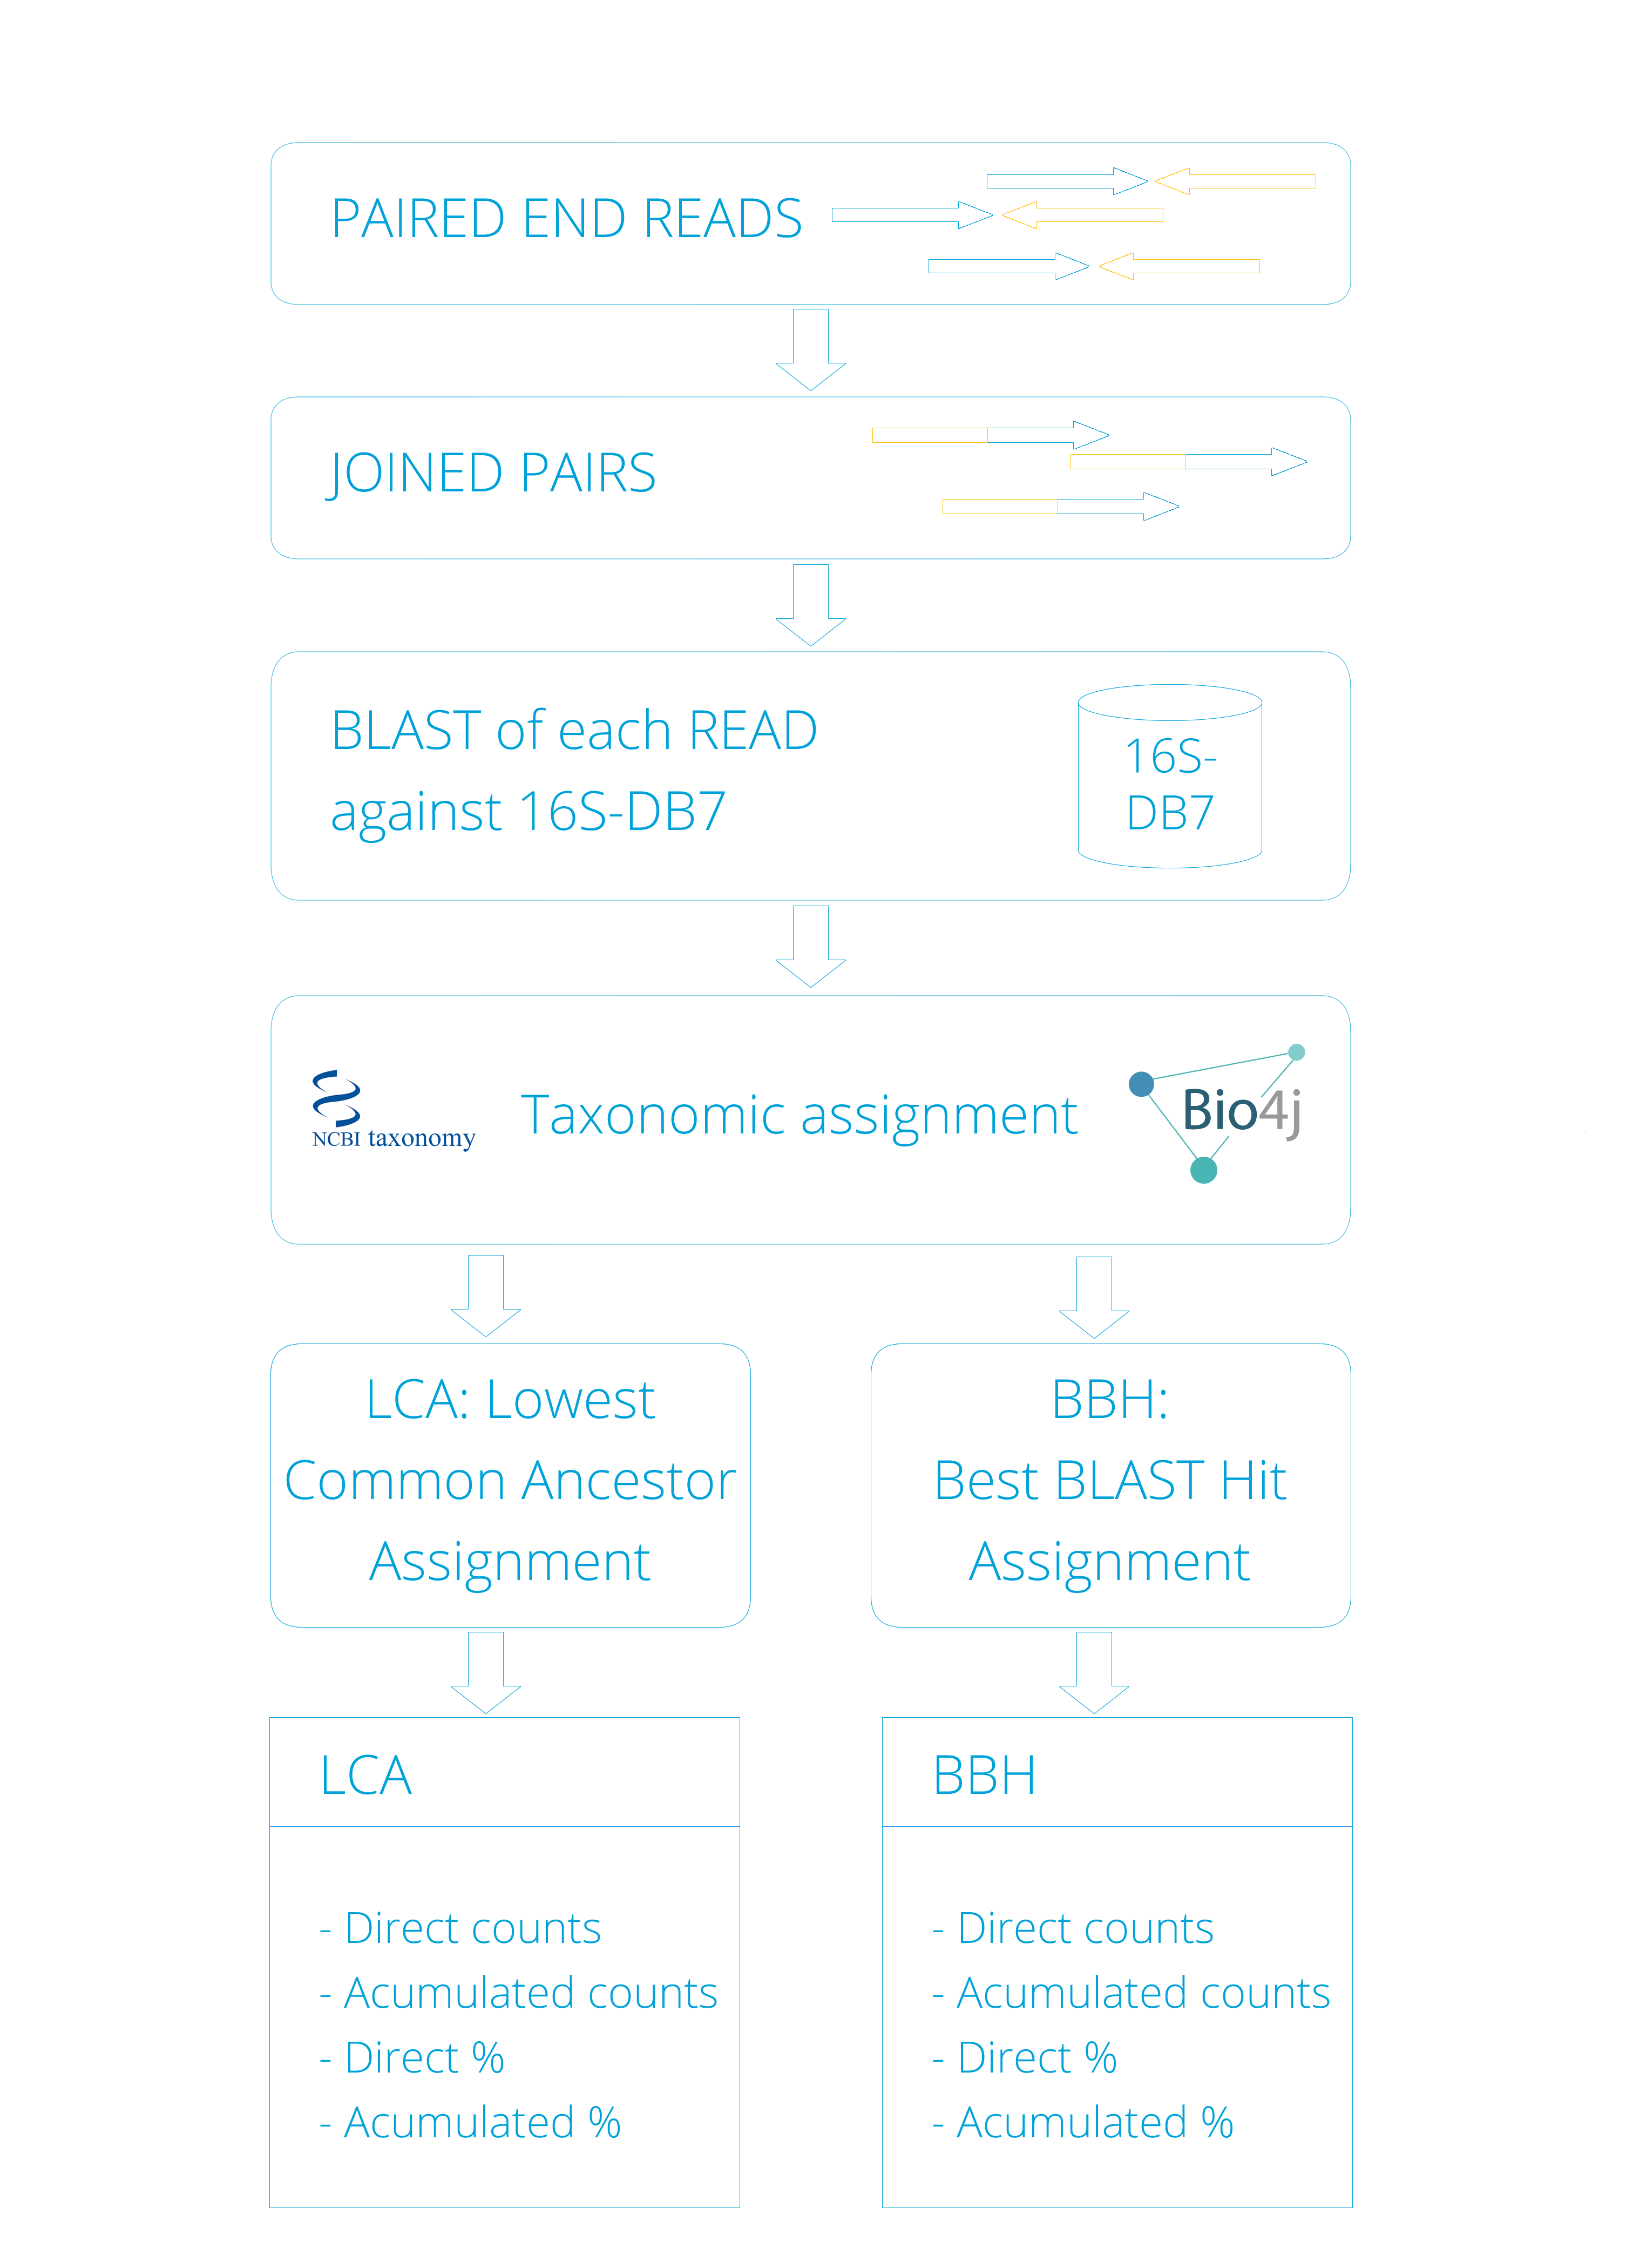
\includegraphics{./Figure-1.jpg}
\caption{\textbf{MG7 analysis workflow.} The paired reads in fastq
format are merged resulting in only one sequence per read pair. The next
step is a parallelized BLASTN of every merged sequence against the 16S
reference database 16S-DB7. Then, the mapping of the detected similar
sequences in the database to the taxonomy node to which they belong is
carried out. This is done using Bio4j that includes a module with all
the NCBI taxonomy in a graph connected with the Gene Ontology, Uniprot,
and RefSeq graphs. Then the taxonomic assignment is done for each
sequence following two different approaches: LCA and BBH, and finally
the abundances corresponding to direct and cumulative assignments for
each node in percentage and absolute counts are provided for each
assignment mode.}
\end{figure}

\subsubsection{Joining reads of each pair using
FLASh}\label{joining-reads-of-each-pair-using-flash}

In the first step the paired-end reads, designed with an insert size
that yields pairs of reads with an overlapping region between them, are
assembled using FLASh \citep{magovc2011flash}. FLASh is designed to
merge pairs of reads when the original DNA fragments are shorter than
twice the length of reads. Thus, the sequence obtained after joining the
2 reads of each pair is larger and has better quality since the sequence
at the ends of the reads is refined merging both ends in the assembly.
To have a larger and improved sequence is crucial to do more precise the
inference of the bacterial origin based on similarity with reference
sequences.

\subsubsection{Parallelized BLASTN of each read against the
16S-DB7}\label{parallelized-blastn-of-each-read-against-the-16s-db7}

The second step is to search for similar 16S sequences in our 16S-DB7
database. The taxonomic assignment for each read is based on BLASTN of
each read against the 16S database.Assignment based on direct similarity
of each read one by one compared against a sufficiently wide database is
considered in different reviews of metagenomics analysis methodologies
\citep{segata2013computational} \citep{morgan2012chapter} as a very
exhaustive method for assignment. Some methods of assignment compare the
sequences only against the 16S genes from available complete bacterial
genomes or avoid computational cost clustering or binning the sequences
first, and then doing the assignments only for the representative
sequence of each cluster. MG7 carries out an exhaustive comparison of
all the reads under analysis and it does not applies any binning
strategy. Every read is specifically compared with all the sequences of
the 16S database. We select the best BLAST hits (10 hits by default)
obtained for each read to do the taxonomic assignment.

\subsubsection{Taxonomic Assignment
Algorithms}\label{taxonomic-assignment-algorithms}

All the reads are assigned under two different algorithms of assignment:
i. Lowest Common Ancestor based taxonomic assignment (LCA) and ii. Best
BLAST Hit based taxonomic assignment (BBH). Figure 2 displays
schematically the LCA algorithm applied sensu stricto (left panel) and
the called `in line' exception (right panel) designed in order to gain
specificity in the assignments in the cases in which the topology of the
taxonomical nodes corresponding to the BLAST hits support sufficiently
the assignment to the most specific taxon.

\begin{figure}[htbp]
\centering
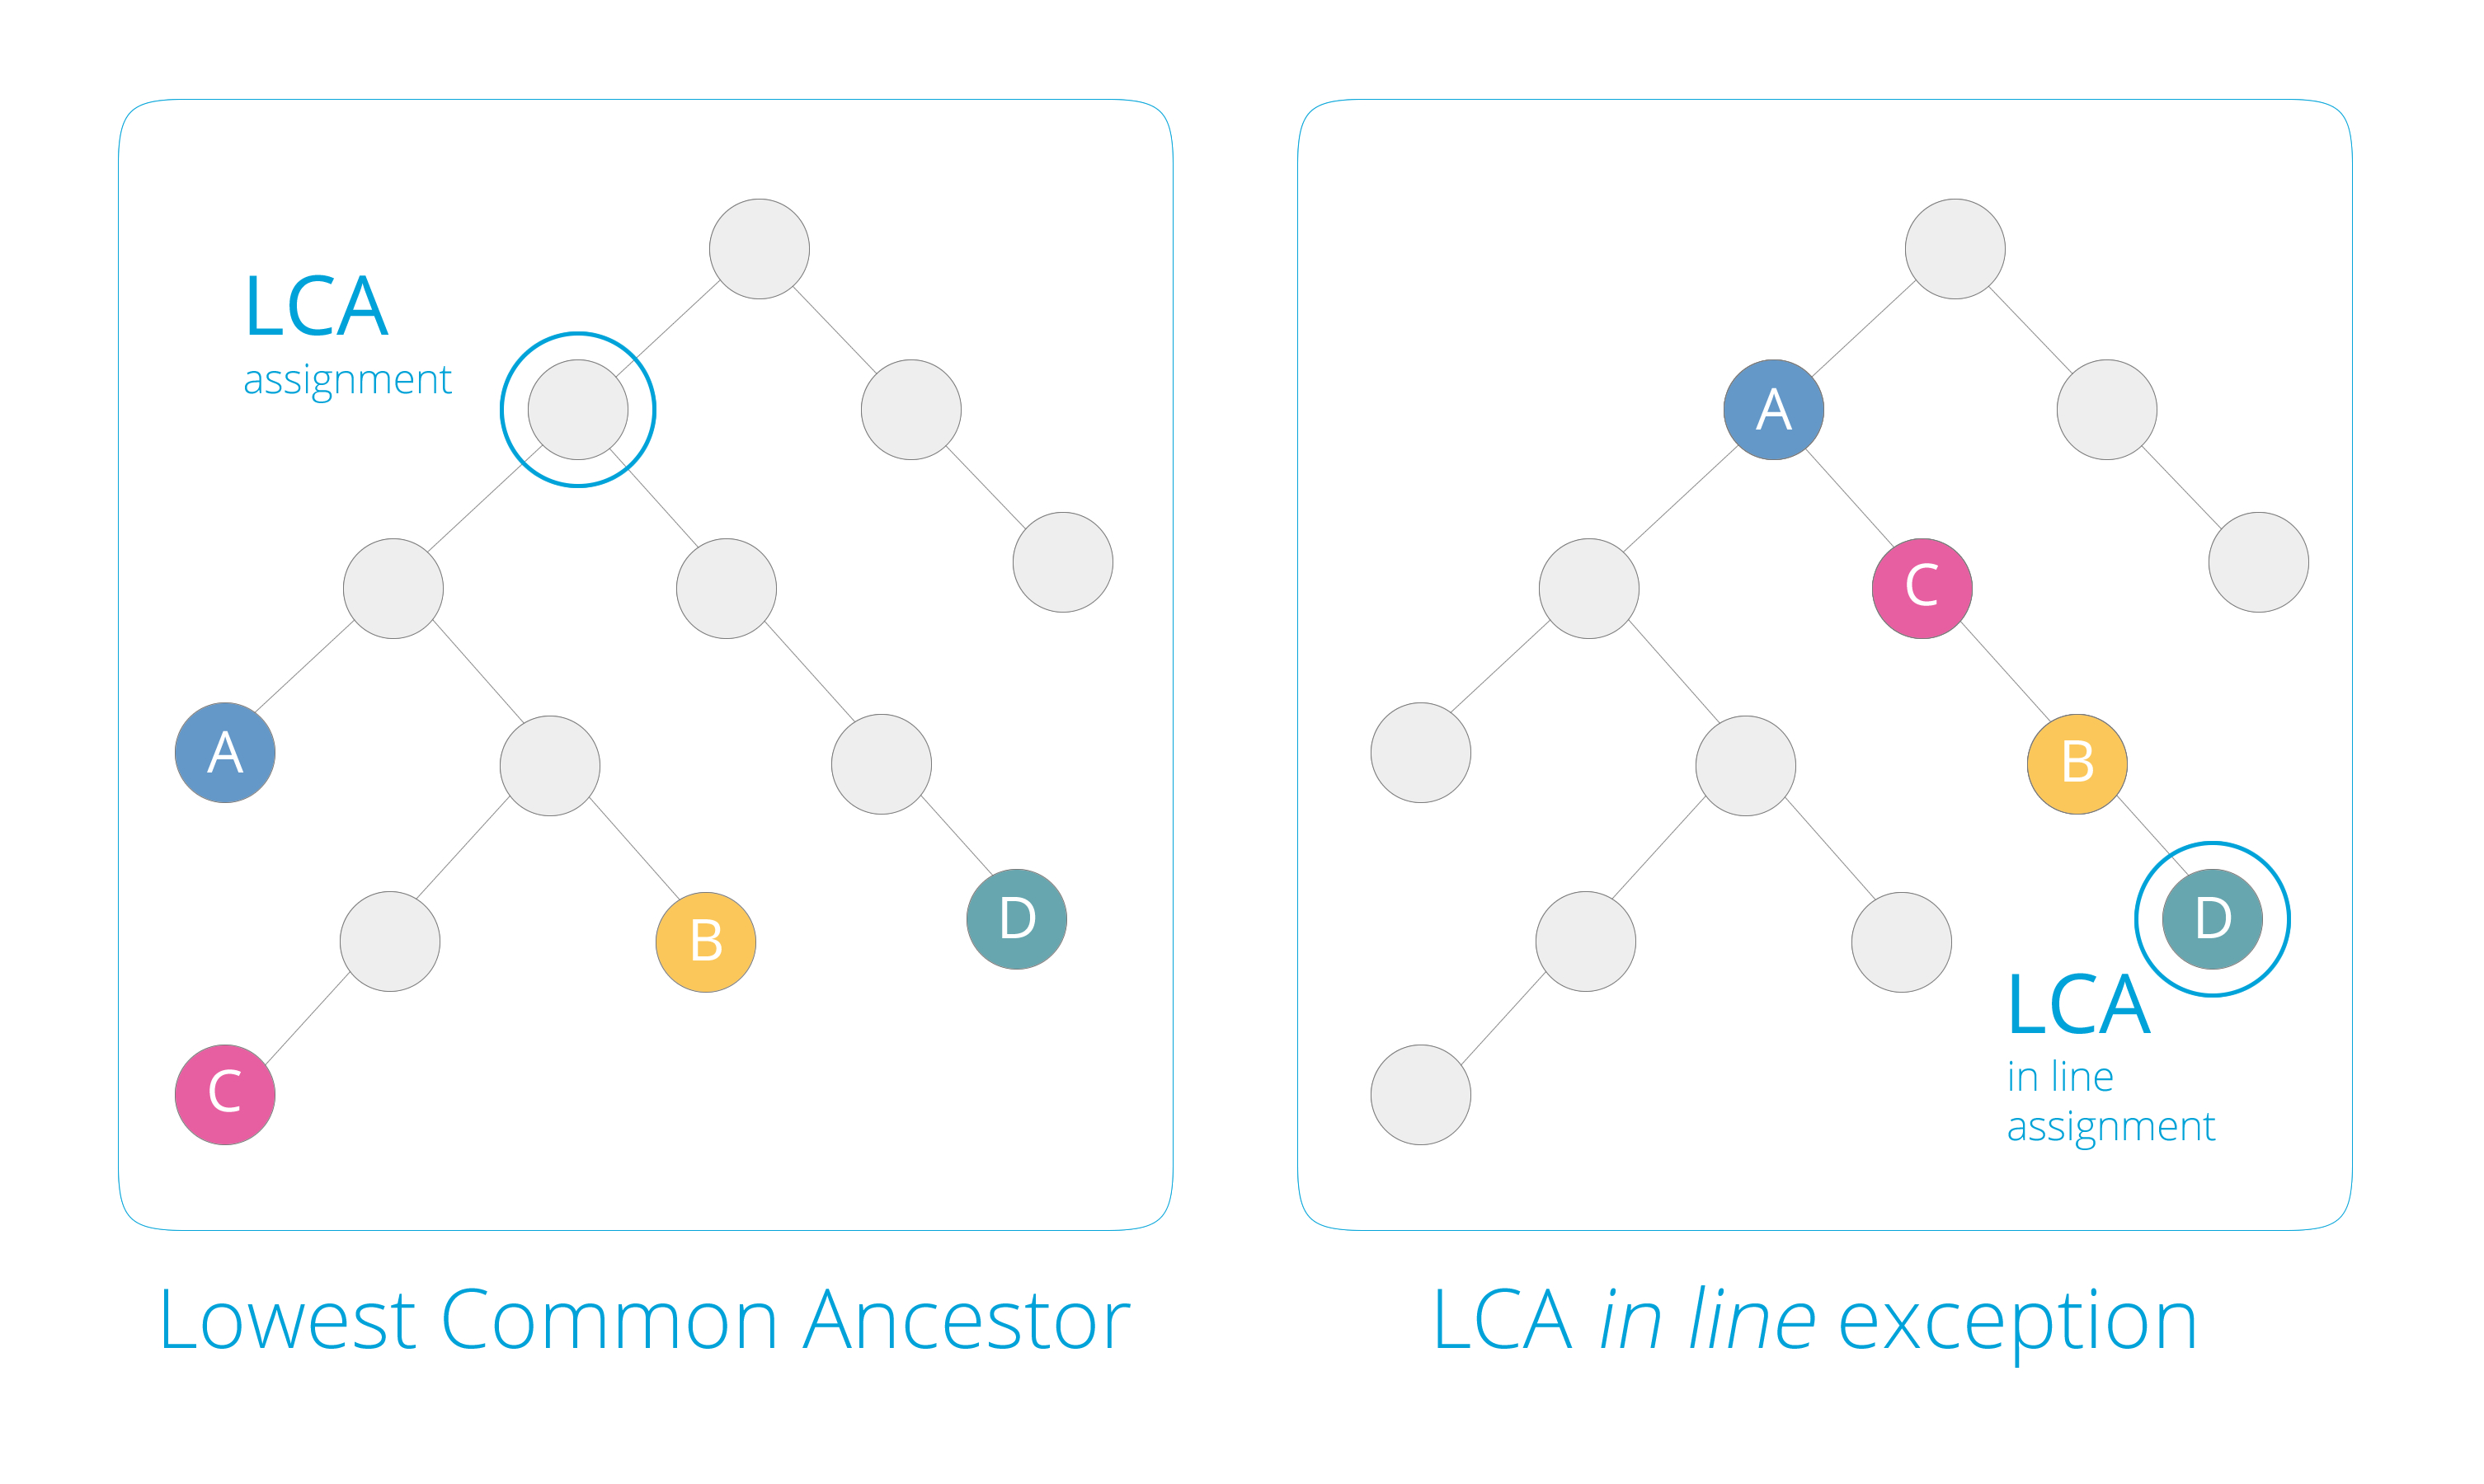
\includegraphics{./Figure-2.jpg}
\caption{\textbf{Lowest Common Ancestor algorithm for taxonomic
assignment.} The Left panel displays an example of the application of
LCA algorithm in a \emph{sensu stricto} mode. A, B, C and D represent
taxonomy tree nodes with assigned reads. Right panel displays the
\emph{in line} mode of assignment which is an exception for the
\emph{sensu stricto} mode of application of LCA algorithm. The \emph{in
line} mode is used when all the nodes are located in a line without
bifurcations. In that case the taxon assigned is the most specific (the
most distant from the root).}
\end{figure}

\paragraph{Lowest Common Ancestor based Taxonomic
Assignment}\label{lowest-common-ancestor-based-taxonomic-assignment}

For each read, first, we select the BEST BLAST HITs (by default 10 Hits)
over a threshold of similarity. To evaluate similarity for this first
filtering of hits we use the Expect value (by default
\(evalue \leq e^{-15}\)) that describes the number of hits one can
``expect'' to see by chance when searching a database of a particular
size. In a second filtering step we filtering those hits that are not
sufficiently good comparing them with the best one. We select the best
HSP (High Similarity Pair) per reference sequence and then choose the
best HSP (that with lowest E-value) between all the selected ones. The
bitscore of this best HSP (called S) is used as reference to filter the
rest of HSPs. All the HSPs with bitscore below the product \(p S\) are
filtered. p is a coefficient fixed by the user to define the bitscore
required, e.g.~if \(p=0.9\) and \(S=700\) the required bitscore
threshold would be \(630\). Once we have the definitive HSPs selected,
we obtain their corresponding taxonomic nodes using the taxonomic
assignments that NCBI provides for all the nt database sequences. Now we
have to analyze the topological distribution of these nodes in the
taxonomy tree: i. If all the nodes forms a line in the taxonomy tree
(are located in a not branched lineage to the tree root) we should
choose the most specific taxID as the final assignment for that read. We
call to this kind of assignment the `in line' exception (see Figure 2
right panel). ii. If not, we should search for the \emph{sensu stricto}
Lowest Common Ancestor (LCA) of all the selected taxonomic nodes (See
Figure 2 left panel). In this approach we decided to use the bitscore
for evaluating the similarity because it is a value that increases when
similarity is higher and depends a lot on the length of the HSP. Some
reads could not find sequences with enough similarity in the database
and then they would be classified as reads with no hits. Advanced
metagenomics analysis approaches \citep{huson2012microbial} have adopted
LCA-based assignment algorithms because it provides fine and trusted
taxonomical assignment.

\paragraph{Best BLAST hit taxonomic
assignment}\label{best-blast-hit-taxonomic-assignment}

We decided to maintain the simpler method of Best BLAST Hit (BBH) for
taxonomic assignment because, in some cases, it can provide information
about the sequences that adds information to that obtained using the LCA
algorithm. With the LCA algorithm, when some reference sequences with
BLAST alignments over the required thresholds map to a not sufficiently
specific taxID, the read can be assigned to an unspecific taxon near to
the root of the taxonomy tree. If the BBH reference sequence maps to
more specific taxa, this method, in that case, gives us useful
information.

\subsubsection{Output for LCA and BBH
assignments}\label{output-for-lca-and-bbh-assignments}

MG7 provides independent results for the 2 different approaches, LCA and
BBH. The output files include, for each taxonomy node (with some read
assigned), abundance values for direct assignment and cumulative
assignment. The abundances are provided in counts (absolute values) and
in percentage normalized to the number of reads of each sample. Direct
assignments are calculated counting reads specifically assigned to a
taxonomic node, not including the reads assigned to the descendant nodes
in the taxonomy tree. Cumulative assignments are calculated including
the direct assignments and also the assignments of the descendant nodes.
For each sample MG7 provides 8 kinds of abundance values: LCA direct
counts, LCA cumu. counts, LCA direct \%, LCA cumu. \%, BBH direct
counts, BBH cumu. counts, BBH direct \% and BBH cumu. \%.

\subsection{Data analysis as a software
project}\label{data-analysis-as-a-software-project}

The MG7 16S data analysis workflow is indeed a set of tasks, all of them
based in \emph{Loquat}. For each task, a set of inputs and outputs as
well as configuration parameters must be statically defined. The user is
also free to leave the reasonable defaults for configuration, needing
only to define the input and output of the whole workflow. The
definition of this configuration is Scala code and the way of starting
an MG7 analysis is compiling the project code and launching it from the
Scala interactive console.

Code compilation prior to launching any analysis assures that no AWS
resources are launched if the analysis is not well-defined, avoiding
expenses not leading to any analysis. Besides compile-time checks,
runtime checks are made before launch to ensure existence of input data
and availability of resources.

An MG7 analysis is then a Scala project where the user only needs to set
certain variables at the code level (input, output and parameters),
compile the code and run it. To facilitate the process of setting up the
Scala project, a template with sensible defaults is provided.

In order to be able to exploit AWS infrastructure for the MG7 analysis,
the user needs to set up an AWS account with certain IAM (Identity and
Access Management) permission policies that will grant access to the
resources used in the workflow.

\subsection{Availability}\label{availability}

MG7 is open source, available at https://github.com/ohnosequences/mg7
under an \href{http://www.gnu.org/licenses/agpl-3.0.en.html}{AGPLv3}
license.

\section{Discussion}\label{discussion}

We could summarize the most innovative ideas and developments in MG7:

\begin{enumerate}
\def\labelenumi{\arabic{enumi}.}
\tightlist
\item
  Treating data analysis as a software project. This makes for radical
  improvements in \emph{reproducibility}, \emph{reuse},
  \emph{versioning}, \emph{safety}, \emph{automation} and
  \emph{expressiveness}
\item
  Checking at compile-time: input and output data, their locations and
  type are expressible and checked at compile-time using \emph{Datasets}
\item
  Management of dependencies and machine configurations using
  \emph{Statika}
\item
  Automation of AWS cloud resources and processes, including
  distribution and parallelization through the use of \emph{Loquat}
\item
  Taxonomic data and related operations are treated natively as what
  they are: graphs, through the use of \emph{Bio4j}
\item
  MG7 provides a sustainable model for taxonomic assignment, appropriate
  to face the challenging amount of data that high throughput sequencing
  technologies generate
\end{enumerate}

We will expand on each item in the following sections.

\subsection{A new approach to data analysis: data analysis as a software
project and checking at
compile-time}\label{a-new-approach-to-data-analysis-data-analysis-as-a-software-project-and-checking-at-compile-time}

MG7 proposes to define and work with a particular data analysis task as
a software project, using Scala. The idea is that \emph{everything}:
data description, their location, configuration parameters and the
infrastructure used should be expressed as Scala code, and treated in
the same way as any (well-managed) software project. This includes,
among other things, using version control systems (\texttt{git} in our
case), writing tests, making stable releases following
\href{http://semver.org/}{semantic versioning} or publishing artifacts
to a repository.

What we see as key advantages of this approach (when coupled with
compile-time specification and checking), are

\begin{itemize}
\tightlist
\item
  \textbf{Reproducibility} the same analysis can be run again with
  exactly the same configuration in a trivial way.
\item
  \textbf{Versioning} as in any software project, there can be different
  versions, stable releases, etc.
\item
  \textbf{Reuse} we can build standard configurations on top of this and
  reuse them for subsequent data analysis. A particular data analysis
  \emph{task} can be used as a \emph{library} in further analysis.
\item
  \textbf{Decoupling} We can start working on the analysis
  specification, without any need for available data in a much easier
  way.
\item
  \textbf{Documentation} We can take advantage of all the effort put
  into software documentation tools and practices, such as in our case
  Scaladoc or literate programming. As documentation, analysis processes
  and data specification live together in the files, it is much easier
  to keep coherence between them.
\item
  \textbf{Expresiveness and safety} For example in our case we can
  choose only from valid illumina read types, and then build a default
  FLASh command based on that. The output locations, being declared
  statically, are also available for use in further analysis.
\end{itemize}

\subsection{Input and output data
declaration}\label{input-and-output-data-declaration}

An important aspect of the MG7 workflow is the way it deals with data
resources. All the data that is going to be used in the analysis or
produced as an output is described as Scala code using rich types from
the \emph{Datasets} language. This allows the user to specify
information about types of data, information that can then be utilized
by tools analyzing this data. For example, we can specify that, for the
first part of the MG7 workflow, running FLASh in parallel requires
illumina paired end reads and produces joined reads.

On one hand, specification of the input data allows us to restrict its
type and force users to be conscious about what they pass as an input.
On the other hand, specification of the output data helps to build a
workflow as a \emph{composition} of several parts: we can ensure on the
Scala code type level that the output of one component fits as an input
for the next component. This is crucial as, obviously, the way a data
analysis task works depends a lot on the particular structure of the
data. For instance, in the MG7 workflow, using BLAST eDSL, we can
precisely describe which format will have the output of the BLAST step,
which information it will include, and then in the next step we can
reuse this description to parse BLAST output and retrieve the part of
the information needed for the taxonomy assignment analysis. Having the
data structure described statically as Scala code allows us to be sure
that we will not have parsing problems or other issues with incompatible
data passed between workflow components.

All this does not compromise flexibility in how the user works with data
in MG7: having static data declarations as a part of the configuration
allows the user to reuse analysis components, or modify them according
to particular needs. Besides that, an important advantage of the
type-level control is the added protection from the execution (and
deployment) of a wrongly configured analysis task, which may lead to
significant costs in both time and money.

\subsection{Tools, data, dependencies and automated
deployment}\label{tools-data-dependencies-and-automated-deployment}

Bioinformatics software often has a complicated installation process and
requires various dependencies with unclear versions. This makes the
deployment of the bioinformatics tools an involved task and resolving it
manually is not a solution in the context of cloud computations. To face
this problem, one needs an automated system of managing tools and
resources, which will allow an expressive way for describing
dependencies between parts of a pipeline and provide a reproducible
procedure of its deployment. We have developed \emph{Statika} for this
purpose and successfully used it in MG7.

Every external tool involved in the workflow is represented as a
\emph{Statika} bundle, which is essentially a Scala project describing
the installation process of this tool and declaring dependencies on
other bundles which will be installed prior to the considered tool
itself. Describing relationships between bundles on the code level
allows us to track the directed acyclic graph of their dependencies and
linearize them to automatically install them sequentially in the right
order. Meanwhile, describing the installation process on the code level
allows the user to utilize the wide range of available Scala and Java
APIs and tools, making installation a well-defined sequence of steps
rather than an unreliable script, dependent on a certain environment.
\emph{Statika} offers an easy path towards making deployment an
automated, reproducible process.

Besides bioinformatics tools like BLAST and FLASh, \emph{Statika}
bundles are used for wrapping data dependencies and all inner components
of the system that require cloud deployment. In particular, all
components of \emph{Loquat} are bundles; the user can then define which
components are needed for the parallel processing on each computation
unit in an expressive way, declaring them as bundle dependencies of the
loquat ``worker'' bundle. This modularization is also important for the
matter of making components of the system reusable for different
projects and liberating the user from most of the tasks related to their
deployment.

\subsection{Parallel computations in the
cloud}\label{parallel-computations-in-the-cloud}

The MG7 workflow consists of certain steps, each of which performs some
work in parallel, using the cloud infrastructure managed by
\emph{Loquat}. It is important to notice the horizontal scalability of
this approach. Irrespectively of how much data needs to be processed,
MG7 will handle it, by splitting data into chunks and performing the
analysis on multiple computation units. The Amazon Elastic Compute Cloud
(EC2) service provides a transparent way of managing computation
infrastructure, called autoscaling groups. The User can set MG7
configuration parameters, adjusting for each task the amount and
hardware characteristics of the EC2 instances they want to use for it.
But it is important to note that, as each workflow step is not very
resource demanding, it is not needed to hire EC2 instances with some
advanced hardware. Instead, an average type will work and you can reduce
execution time by simply scaling out the number of instances.

\subsection{Taxonomy and Bio4j}\label{taxonomy-and-bio4j}

The hierarchic structure of the taxonomy of the living organisms is a
tree, and, hence, is also a graph in which each node, with the exception
of the root node, has a unique parent node. It led us to model the
taxonomy tree as a graph using the graph database paradigm. Previously
we developed Bio4j \citep{pareja2015bio4j}, a platform for the
integration of semantically rich biological data using typed graph
models. It integrates most publicly available data linked with sequences
into a set of interdependent graphs to be used for bioinformatics
analysis and especially for biological data. MG7 works based on the
Bio4j taxonomy module. It opens the possibility to connect the taxonomic
profiling data obtained with MG7 to all the biological knowledge
associated to each taxon. Using the information available in Bio4j for
all the proteins assigned to each taxon we are connected to all the
functional data available in Uniprot related with it.

\subsection{Future developments}\label{future-developments}

\subsubsection{Shotgun metagenomics}\label{shotgun-metagenomics}

It is certainly possible to adapt MG7 to work with shotgun metagenomics
data. Simply changing the reference database to include whole genome
sequence data could yield interesting results. This could also be
refined by restricting reference sequences according to all sort of
criteria, like biological function or taxonomy. Bio4j would be an
invaluable tool here, thanks to its ability to express complex
predicates on sequences using all the information linked with them (GO
annotations, UniProt data, NCBI taxonomy, etc).

\subsubsection{Comparing groups of
samples}\label{comparing-groups-of-samples}

The comparison of the taxonomic profiles between different groups of
samples is a need for many metagenomics studies. Tasks related with this
group-based analysis, such as the extraction of the minimal tree with
all the taxa with some direct or accumulated assignment, will be part of
a new MG7 module, already in development.

\subsubsection{Interactive visualizations based on
Biographika}\label{interactive-visualizations-based-on-biographika}

New visualization tools for metagenomics results are undoubtedly needed.
Interactivity is a especially interesting feature for metagenomics data
visualization, since the expert needs to explore the results in a
knowledge-driven way. The majority of the available metagenomics data
visualizations are static. We are working in the \emph{Biographika}
project \citep{tobes2015biographika}, to provide interactive rich
visualizations on the web for Bio4j data. The development of
visualizations specific for MG7 is one of Biographika current goals.
Biographika is based on D3.js, the de-facto standard JavaScript data
visualization library, and is open source.

\section{Materials and Methods}\label{materials-and-methods}

\subsection{Amazon Web Services}\label{amazon-web-services}

MG7 uses the following Amazon Web Services:

\begin{itemize}
\tightlist
\item
  \href{https://aws.amazon.com/ec2}{EC2} (Elastic Compute Cloud)
  autoscaling groups for launching and managing computation units
\item
  \href{https://aws.amazon.com/s3}{S3} (Simple Storage Service) for
  storing input and output data
\item
  \href{https://aws.amazon.com/sqs}{SQS} (Simple Queue Service) for
  communication between different components of the system
\item
  \href{https://aws.amazon.com/sns}{SNS} (Simple Notification Service)
  for e-mail notifications
\end{itemize}

These services are used through a Scala wrapper of the official
\href{https://aws.amazon.com/sdk-for-java/}{AWS Java SDK v1.9.25}:
\href{https://github.com/ohnosequences/aws-scala-tools/releases/tag/v0.13.2}{ohnosequences/aws-scala-tools
v0.13.2}.

\subsection{Scala}\label{scala}

MG7 itself and all the libraries used are written in Scala v2.11.

\subsection{Statika}\label{statika}

MG7 uses
\href{https://github.com/statika/statika/releases/tag/v0.2.0}{ohnosequences/statika
v2.0.0} for specifying the configuration and behavior of EC2 instances.

\subsection{Datasets}\label{datasets}

MG7 uses
\href{https://github.com/ohnosequences/datasets/releases/tag/v0.2.0}{ohnosequences/datasets
v0.2.0} for specifying input and output data, their type and their
location.

\subsection{Loquat}\label{loquat}

MG7 uses
\href{https://github.com/ohnosequences/loquat/releases/tag/v2.0.0}{ohnosequences/loquat
v2.0.0} for the specification of data processing tasks and their
execution using AWS resources.

\subsection{BLAST eDSL}\label{blast-edsl}

MG7 uses
\href{https://github.com/ohnosequences/blast/releases/tag/v0.2.0}{ohnosequences/blast
v0.2.0}. The BLAST version used is v2.2.31+.

\subsection{FLASh eDSL}\label{flash-edsl}

MG7 uses
\href{https://github.com/ohnosequences/flash/releases/tag/v0.1.0}{ohnosequences/flash
v0.1.0}. The FLASh version used is v1.2.11.

\subsection{Bio4j}\label{bio4j}

MG7 uses
\href{https://github.com/bio4j/bio4j/releases/tag/v0.12.0-RC3}{bio4j/bio4j
v0.12.0-RC3} and
\href{https://github.com/bio4j/bio4j-titan/releases/tag/v0.4.0-RC2}{bio4j/bio4j-titan
v0.4.0-RC2} as an API for the NCBI taxonomy.

\section{Disclosure/Conflict-of-Interest
Statement}\label{disclosureconflict-of-interest-statement}

All authors work at the \emph{Oh no sequences!} research group, part of
Era7 Bioinformatics. Era7 offers metagenomics data analysis services
based on MG7. MG7 is open source, available under the OSI-approved
AGPLv3 license.

\section{Author Contributions}\label{author-contributions}

\begin{itemize}
\tightlist
\item
  \textbf{AA} developed \emph{MG7}, \emph{Statika}, \emph{Datasets}, and
  \emph{aws-scala-tools}; wrote the paper;
\item
  \textbf{EK} developed \emph{nispero} (a prototype for \emph{Loquat}
  \citep{kovach2014nispero}) and \emph{aws-scala-tools}.
\item
  \textbf{MM} \emph{MG7} workflow design; curation and design of the
  \emph{16S-DB7} reference database; wrote the paper.
\item
  \textbf{PPT} curation, design, data extraction code of the
  \emph{16S-DB7} reference database.
\item
  \textbf{EP} \emph{MG7} workflow design; wrote the paper.
\item
  \textbf{RT} \emph{MG7} workflow design, assignment strategy; curation
  and design of the \emph{16S-DB7} reference database; wrote the paper.
\item
  \textbf{EPT} developed \emph{MG7}, \emph{Statika}, \emph{Datasets},
  \emph{FLASh/BLAST eDSLs}; data analysis approach and design; wrote the
  paper.
\end{itemize}

All authors have read and approved the final manuscript.

\section{Acknowledgements}\label{acknowledgements}

\emph{Funding:} The two first authors are funded by INTERCROSSING (Grant
289974).

  
\bibliography{./out/../refs}

\end{document}
